\documentclass{article}

\usepackage{fullpage,amsmath,amsthm,graphicx,enumitem}
\usepackage{hyperref}
\usepackage{amssymb}
\usepackage{wasysym}
\usepackage{empheq}

\theoremstyle{definition}
\newtheorem{question}{Question}

\newcommand{\option}{{\Large$\Square$ }}
\def\IfSoln#1{\IfFileExists{solutions/#1}{\input{solutions/#1}}{}}

\title{ASEN 3728 Aircraft Dynamics\\Written Homework 4}

\date{Due date listed on Gradescope.}

\begin{document}

\maketitle

\begin{question}

For this problem \underline{assume the thrust is equal and opposite to the drag}. Consider an aircraft with the following parameters
\begin{table}[!h]
\centering
%\caption{Aircraft parameters}
\label{my-label}
\begin{tabular}{llll}
 m = 6.77 kg & c = 0.2 m   & b = 3.3 m \\
 S = 0.67 m$^2$ & $C_{D_\text{min}}$ = 0.02  &  K = 0.0224   \\
 $C_{L_{\alpha}}$ = 5.75 & $C_{L_{q}}$ = 10.14  & $C_{L_{\delta_e}}$ = 0.0079  \\
 $C_{m_{q}}$ = -24.4  & $C_{m_{\delta_e}}$ = -0.02  & $C_{m_{\text{zero}}}$ = 0.12\\
 $C_{L_\text{min}} = 0$ & & 
\end{tabular}
\end{table}

\begin{enumerate}
\item What is the drag coefficient of the aircraft when at trim with density $\rho$ = 1.10 kg/m$^3$ and airspeed $V_a$ = 21 m/s?

\item Consider an aircraft flying with with the same airspeed and density above. You wish to put the aircraft in trim with $\delta_e = 1.65^{\circ}$ and $\alpha = 4.07^{\circ}$. These values balance the forces but not the moment. You are allowed to change the location $h$ of the center of gravity. If the neutral point $h_n$ = 0.75, where must you locate the center of gravity of the aircraft for it to be in trim?
\end{enumerate}
\end{question}

\vspace{0.1cm}
\clearpage

\vspace{0.1cm}

\begin{question} Consider an aircraft cruising at an airspeed of 176 ft/s with the following longitudinal dynamics matrix for longitudinal perturbation state $\Delta \mathbf{x} = [ \Delta u, \Delta w, \Delta q, \Delta \theta ]^T$ and control input $\delta_e$:
\[
A_{\text{lon}} = \begin{bmatrix}
-0.045 & 0.036 & 0 & -32.2 \\
-0.369 & -2.02 & 176 & 0 \\
0.0019 & -0.0396 & -2.948 & 0 \\
0 & 0 & 1 & 0
\end{bmatrix} \quad \quad B_{\delta_e} = \begin{bmatrix}
0 \\
-28.2 \\
-11.9 \\
0 
\end{bmatrix}
\]
where all units are English.

\begin{enumerate}

    % \item If the aircraft is operating at trim, except that its speed is 186 ft/s ($\Delta u = 10$ ft/s), what is the acceleration in the body x-direction, $\Delta \dot{u}\,$? Assume no control input.
    \item If the aircraft is operating near trim at $\Delta \mathbf{x} = [10\,\text{ft/s}, 0, 0, 0]^T$, what is the acceleration in the body x-direction, $\Delta \dot{u}\,$? Assume no control input.

\item Calculate the eigenvalues of $A_\text{lon}$. Indicate which eigenvalues correspond to the short period and phugoid modes of the aircraft. Briefly justify your answer.

\item Consider the control law $\delta_e = -k_1 \, \Delta q - k_2 \, \Delta \alpha$. Determine what the gain matrix $K$ should be so that $A^{cl} = A_{\text{lon}} - B_{\delta_e} K$ would be the closed-loop dynamics matrix for the controlled system. The final answer should be $K$ and should include entries with $k_1$, $k_2$, and possibly other quantities; you do not need to write out $A^{cl}$.

% \item If a perturbation was applied, would the aircraft return to trim if no controls were utilized? Consider longitudinal dynamics and justify your answer.

\item Calculate the eigenvalues of the closed-loop dynamics matrix $A^{cl}$ using values of $k_1 = 0.1$ and $k_2 = 0.5$ in the control law from part 3. By what percentage do the natural frequencies of the short period and phugoid modes change between the open-loop and closed-loop dynamics using these gain values?


% \item Determine an initial condition such that the initial perturbation in $\Delta q$ is maximized in the phugoid mode. 
% \item Derive an expression for the dynamic response of the aircraft's pitch rate $\Delta q(t)$. 
% 
% \item How does the change in $\Delta q$ shortly following the perturbation effect the lift force if $C_{L_q} = 8.75$? Justify your answer.
\end{enumerate}
\end{question}
\clearpage

\vspace{6cm}

\begin{question}
Consider an aircraft with mass and geometric properties given in Table 1, flying at a trim condition described by Table 2. Assume the aircraft has a constant-power engine and the thrust is aligned with the body x-axis, i.e. the thrust IS NOT opposite the drag.

\begin{itemize}
\item Determine the lift and drag coefficients of the aircraft in trim. It may be helpful to draw a free body diagram of the aircraft.
\item Calculate the dimensional stability derivatives $Z_w$, $X_w$, and $M_w$.
%\item Determine the dimensional stability derivatives $Z_u$, $X_u$, and $M_u$.
\end{itemize}

\begin{table}[ht] 
\caption{Mass and Geometric Properties} % title of Table 
\centering % used for centering table 
\begin{tabular}{| c | c | c | c | c | c | c | c |} % centered columns (4 columns) 
\hline %inserts double horizontal lines 
Variable & Value & & Variable & Value & & Variable & Value\\ [0.5ex] % inserts table 
%heading 
\hline % inserts single horizontal line 
$m$ & 22,000 kg & & $S$ & 87 m$^2$ & & $c$ & 3.9 m \\
$b$ & 22.3 m & & $a_{wb}$ & 4.4/rad & & static margin & .25 \\
$S_t$ & 21.4 m$^2$ & & $\partial \epsilon / \partial \alpha$ & 0.3 & & $a_{t}$ & 3.67/rad \\
$e$ & 0.95 & & & & & &\\

\hline %inserts single line 
\end{tabular} 
\label{table:nonlin} % is used to refer this table in the text 
\end{table}

\begin{table}[ht] 
\caption{Trim condition} % title of Table 
\centering % used for centering table 
\begin{tabular}{| c | c | c | c | c | c | c | c |} % centered columns (4 columns) 
\hline %inserts double horizontal lines 
Variable & Value & & Variable & Value & & Variable & Value \\ [0.5ex] % inserts table 
%heading 
\hline % inserts single horizontal line 
$\rho_0$ & 1.225 kg/m$^3$ & & $\alpha_0$ & $1.2^{\circ}$ & & $u_0$ & 125 m/s \\
$\gamma_{a_0}$ & 0 & & thrust $T_0$ & 14,000 N & &  & \\
\hline %inserts single line 
\end{tabular} 
\label{table:nonlin} % is used to refer this table in the text 
\end{table}
\end{question}

\vspace{0.1cm}

\clearpage

\begin{question}
    Consider an aircraft with a canard, such that the aircraft has no tail, but has a control surface forward of the wings, as shown below. Assume the canard (shown in red) and the center of gravity are at the same vertical height relative to the zero lift line. You may also assume that $V=u_0$.

    \begin{figure}[h]
        \centering
        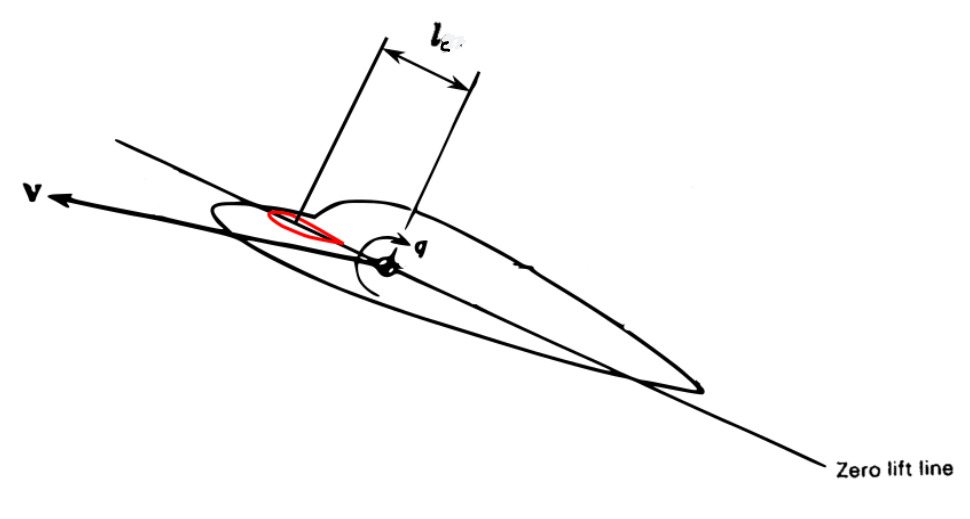
\includegraphics[width=0.5\textwidth]{questions/canard.png}
        % \caption{Caption}
        \label{fig:canard}
    \end{figure}

    The pitching moment coefficient for the canard $C_{m_c}$ is
    \begin{equation*}
        C_{m_c} = \frac{l_cS_c}{\bar{c}S}C_{l_c}=V_{H_c}C_{l_c},
    \end{equation*}
    where $S_c$ is the area of the canard, $S$ is the area of the wing, $l_c$ is the distance between the CG and the canard mean aerodynamic center, $\bar{c}$ is the length of the mean aerodynamic chord, and $V_{H_c}$ is the canard volume ratio.

\begin{enumerate}
    \item Use a diagram to determine $\Delta \alpha_c$, the change in the effective angle of attack for the canard, as a function of $q$.
    \item Find $(C_{m_q})_{\text{canard}}$, the canard contribution to the pitching moment stability derivative.
\end{enumerate}

\end{question}

\vspace{0.1cm}

\end{document}